%; whizzy paragraph -pdf xpdf -latex ./whizzypdfptex.sh
%; whizzy-paragraph "^\\\\begin{frame}"
% latex beamer presentation.
% platex, latex-beamer でコンパイルすることを想定。 

%     Tokyo Debian Meeting resources
%     Copyright (C) 2009 Junichi Uekawa
%     Copyright (C) 2009 Nobuhiro Iwamatsu

%     This program is free software; you can redistribute it and/or modify
%     it under the terms of the GNU General Public License as published by
%     the Free Software Foundation; either version 2 of the License, or
%     (at your option) any later version.

%     This program is distributed in the hope that it will be useful,
%     but WITHOUT ANY WARRANTY; without even the implied warreanty of
%     MERCHANTABILITY or FITNESS FOR A PARTICULAR PURPOSE.  See the
%     GNU General Public License for more details.

%     You should have received a copy of the GNU General Public License
%     along with this program; if not, write to the Free Software
%     Foundation, Inc., 51 Franklin St, Fifth Floor, Boston, MA  02110-1301 USA

\documentclass[cjk,dvipdfmx,12pt]{beamer}
\usetheme{Tokyo}
\usepackage{monthlypresentation}

%  preview (shell-command (concat "evince " (replace-regexp-in-string "tex$" "pdf"(buffer-file-name)) "&")) 
%  presentation (shell-command (concat "xpdf -fullscreen " (replace-regexp-in-string "tex$" "pdf"(buffer-file-name)) "&"))
%  presentation (shell-command (concat "evince " (replace-regexp-in-string "tex$" "pdf"(buffer-file-name)) "&"))

%http://www.naney.org/diki/dk/hyperref.html
%日本語EUC系環境の時
\AtBeginDvi{\special{pdf:tounicode EUC-UCS2}}
%シフトJIS系環境の時
%\AtBeginDvi{\special{pdf:tounicode 90ms-RKSJ-UCS2}}

\title{Debian勉強会の資料のePUB化を試みた}
\subtitle{}
\author{まえだこうへい}
\date{2013年8月17日}
\logo{\includegraphics[width=8cm]{image200607/openlogo-light.eps}}

\begin{document}

\frame{\titlepage{}}

\begin{frame}
\begin{center}
{\Huge eBook使ってます?}
\end{center}
\end{frame}

\begin{frame}{ePUB化の動機}
 \begin{itemize}
  \item[when:] ePUBフォーマットの書籍購入し始めたころから
  \item[why:] PDFだとフォントサイズの変更でページが自動的にリサイズされない\footnote{特にスマホとか不便}
  \item[how:] Debian勉強会の資料のHTML版を変換すれば楽そう\footnote{\url{http://tokyodebian.alioth.debian.org/html/}}
 \end{itemize}
\end{frame}

\begin{frame}{今回ePUB化を試すにあたり}
  \begin{itemize}
  \item Debian勉強会資料のHTML化の方法が不明(一昨日見つけた)
  \item \LaTeX から直接変換できた方が流れはきれい
  \item \LaTeX → DVI → PDF のどこからでもePUB化はできるのではないか?と思って調べてみた
  \end{itemize}
\end{frame}


\begin{frame}{\LaTeX から ePUB への変換のフロー}
\begin{figure}[H]
\begin{center}
  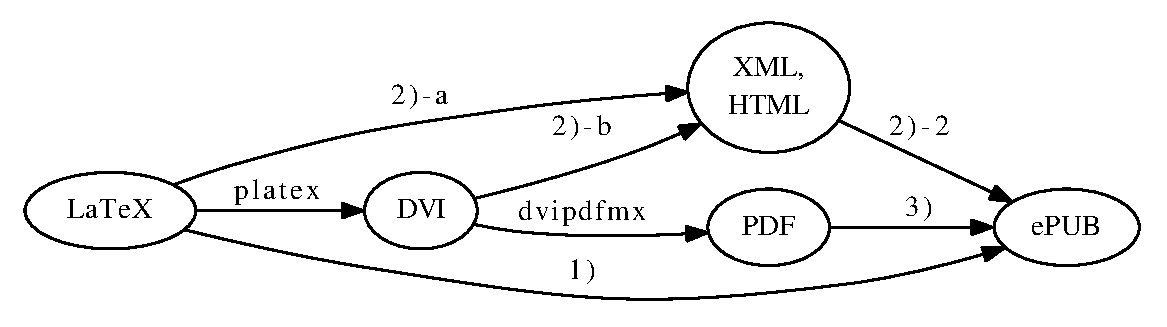
\includegraphics[width=1.0\hsize]{image201308/latex-epub.eps}
 \label{fig:convert-latex-to-epub}
\end{center}
\end{figure}
\end{frame}

\begin{frame}{検証したツールとその結果}
\begin{center}
{\small
\begin{tabular}{|c|c|c|c|c|c}
\hline
パターン & ツール名 & 入力 & 出力 & \multicolumn{2}{|c|}{結果} \\ \cline{1-4}
 & & & & A\footnote{{\scriptsize Debian勉強会の資料}} & B\footnote{{\scriptsize latex2epubのサンプル}} \\
\hline
1) & Pandoc\footnote{{\scriptsize input/outputとも様々なフォーマットに対応した変換ツール}} & \LaTeX & ePUB & NG & OK \\
1) & latex2epub\footnote{{\scriptsize 武藤さんが作成したツール}} & \LaTeX & ePUB & NG & OK \\
2)-a & \LaTeX ML & \LaTeX & XML & NG & OK \\
2)-b & \TeX4ht & DVI & HTML & NG & NG \\
2)-b & htplatex\footnote{{\scriptsize 上川さんが作成したDebian勉強会のHTML化スクリプト}}(\TeX4ht) & \TeX & HTML & \textcolor{blue}{OK} & NG \\
3) & Pandoc & HTML & ePUB & \textcolor{blue}{OK} & N/A \\
4) & Calibre & PDF & ePUB & \textcolor{blue}{OK} & OK \\
\hline
\end{tabular}
}
\end{center}
\end{frame}

\begin{frame}{生成されたePUBは?}
  htplatex \& Pandocの場合
 \begin{itemize}
   \item 表示が崩れる箇所あり
     \begin{itemize}
     \item tabularがtableに変換されず、表にならない
     \item 表紙の画像が追加されない
     \end{itemize}
   \item \TeX4ht で追加されるナビゲートのメニューが残る
  \item 夏・冬号が含む月の資料よりも先に変換すると、その中の画像がコピーされず、pandoc実行時に失敗する
  \item \TeX4htでHTML変換時に自動生成される画像のファイル名が異なり、pandoc実行時に失敗することがある
 \end{itemize}
\end{frame}

\begin{frame}{生成されたePUBは?}
  Calibreの場合
\begin{itemize}
  \item 目次のレイアウトが崩れる
  \item デフォルトでは行間が広すぎる
  \item 図が表示されない場合もある
  \item tabularが表として表示されない
\end{itemize}
変換時に次のオプションを入れると多少マシ。
\begin{itemize}
  \item "ヒューリスティック処理を有効にする"
  \item "外観"→"段落の間の間隔を削除する"
\end{itemize}
\end{frame}

\begin{frame}{他のサンプルや他のツールでの検証}

{\scriptsize
  \begin{itemize}
  \item pandocで \LaTeX を変換した場合
    \begin{itemize}
    {\scriptsize
    \item \texttt{\textbackslash includegraphics}がimageという文字列になったり、
    \item \texttt{\textbackslash underline}の中が表示されない
    \item \texttt{\textbackslash multicol, \textbackslash newpage, \textbackslash minipage}など未対応
    \item \texttt{\textbackslash dancersectionなどのマクロ展開できない}
    \item セクションタイトルが文字化け
    \item listingでもコードブロックがうまく表示されず
}
    \end{itemize}
  \item \LaTeX ML は\texttt{\textbackslash commandline}がダメ
  \item latex2html はjsarticleは未対応。utf8にしたら日本語 \LaTeX でも変換できるがHTMLの出力は文字化け(charsetが入らないため。エンコード指定すれば表示される)
  \item Hermes\footnote{\url{http://hermes.roua.org/}} はフォント関連のエラー
  \item ePUB readerでも、fbreaderなら画像表示されるのにCalibreでは表示されなかったり
\end{itemize}
}
\end{frame}

\begin{frame}[containsverbatim]{htplatex \& pandocでの変換用スクリプト}
\begin{commandline}
$ sudo apt-get install dvi2ps-fontdata-a2n dvi2dvi \
  dvipng pandoc
$ htplatex -e debianmeetingresume201308.tex \
  jp,2,sections+
$ ls epub/
debianmeetingresume201308.epub
\end{commandline}
※PDFをビルドするときは、dvi2ps-fontdata-a2nをアンインストールしておくこと。
\end{frame}

\begin{frame}{まとめ}
\begin{itemize}
  \item \LaTeX を使っていても、 Debian勉強会とそれ以外では同じやり方で変換できるわけではない
  \item Debian勉強会の資料をePUB化には、htplatex でのHTMLの編集の調整が必要
    \begin{itemize}
    \item \TeX 4ht コマンド(\texttt{\textbackslash HChar}や\texttt{\textbackslash HCode}を指定している箇所など)のカスタマイズなど\footnote{\url{http://osksn2.hep.sci.osaka-u.ac.jp/~naga/miscellaneous/tex4ht/tex4ht-howtose4.html\#x5-150004.3}}
    \item Calibre はGUI \& 変換のカスタマイズの自由度が低いので無理ゲー
    \end{itemize}
  \item 最初からPDFおよびePUB生成に対応したドキュメントジェネレータ(例えば、ReVIEW\footnote{\url{https://github.com/kmuto/review}})に切り替える、というのも手段としてはあるけど、どうなんでしょうね。
\end{itemize}
\end{frame}

\end{document}
